\documentclass[12pt, a4paper]{report}

% ==========================================
% PACKAGES
% ==========================================
\usepackage[utf8]{inputenc}
\usepackage[french]{babel}
\usepackage[T1]{fontenc}
\usepackage{graphicx}
\usepackage{geometry}
\usepackage{hyperref}
\usepackage{setspace}
\usepackage{titlesec}
\usepackage{xcolor}
\usepackage{float}
\usepackage{tikz}
\usepackage{colortbl}
\usepackage{listings}
\usepackage{fancyhdr}
\usetikzlibrary{shapes.geometric, arrows, positioning}

% Configuration des couleurs des titres (Demande personnalisée)
\definecolor{MonVert}{RGB}{34, 139, 34} % Un vert lisible (Forest Green)

\titleformat{\chapter}[display]
  {\normalfont\huge\bfseries\color{red}}
  {\chaptertitlename\ \thechapter}{20pt}{\Huge}
  
\titleformat{\section}
  {\normalfont\Large\bfseries\color{MonVert}}
  {\thesection}{1em}{}

\titleformat{\subsection}
  {\normalfont\large\bfseries\color{MonVert}}
  {\thesubsection}{1em}{}
  
\titleformat{\subsubsection}
  {\normalfont\normalsize\bfseries\color{MonVert}}
  {\thesubsubsection}{1em}{}

% Configuration de la page
\geometry{top=2.5cm, bottom=2.5cm, left=3cm, right=2.5cm}
\onehalfspacing

% ==========================================
% EN-TÊTE ET PIED DE PAGE (Sur toutes les pages)
% ==========================================
\pagestyle{fancy}
\fancyhf{} % Nettoie les anciens headers/footers
\fancyhead[L]{\textit{Rapport de Stage de Fin d'Études}}
\fancyhead[R]{\textbf{BTS DAI}}
\fancyfoot[L]{Rayan El Habib}
\fancyfoot[C]{Prestige Maroc}
\fancyfoot[R]{Page \thepage}
\renewcommand{\headrulewidth}{0.4pt} % Ligne sous l'en-tête
\renewcommand{\footrulewidth}{0.4pt} % Ligne au-dessus du pied de page

% Styles TikZ
\tikzstyle{process} = [rectangle, minimum width=3cm, minimum height=1cm, text centered, draw=black, fill=blue!10, rounded corners]
\tikzstyle{database} = [cylinder, shape border rotate=90, aspect=0.25, draw, minimum height=2cm, minimum width=1.5cm, fill=green!10, text centered]
\tikzstyle{actor} = [circle, draw=black, fill=orange!10, minimum size=1.5cm, text centered]
\tikzstyle{arrow} = [thick,->,>=stealth]
\tikzstyle{usecase} = [ellipse, draw=black, fill=yellow!20, minimum width=3cm, text centered]
\tikzstyle{line} = [draw, thick, -]

\begin{document}

% 00. Pages préliminaires
\begin{titlepage}
    \begin{center}
        % Logos
        \begin{minipage}{0.45\textwidth}
            \begin{flushleft}
                
\includegraphics[height=2.5cm]{"images/bts alekenyd.jpg"}
            \end{flushleft}
        \end{minipage}
        \hfill
        \begin{minipage}{0.45\textwidth}
            \begin{flushright}
                
\includegraphics[height=2.5cm]{images/Prestigemaroc.png}
            \end{flushright}
        \end{minipage}
        
        \vspace*{0.5cm}
        \large \textbf{MINISTÈRE DE L'ENSEIGNEMENT SUPÉRIEUR} \\
        \textbf{ÉTABLISSEMENT ALKENDI}
        
        \vspace{1cm}
        \Large \textbf{RAPPORT DE STAGE DE FIN D'ÉTUDES} \\
        \normalsize Pour l'obtention du \textbf{Brevet de Technicien Supérieur (BTS)} \\
        \normalsize \textbf{Filière : Développement d'Applications Informatiques (DAI)}
        
        \vspace{1.5cm}
        \rule{\linewidth}{0.5mm} \\[0.4cm]
        \huge \textbf{Conception, Architecture et Développement d'un Écosystème Numérique Unifié :} \\[0.2cm]
        \LARGE \textbf{Service Location, Service ERP et Service CRM} \\[0.4cm]
        \rule{\linewidth}{0.5mm}
        
        \vfill
        
        \begin{minipage}{0.45\textwidth}
            \begin{flushleft}
                \large \textbf{Réalisé par :} \\
                \textbf{Rayan El Habib}
            \end{flushleft}
        \end{minipage}
        \hfill
        \begin{minipage}{0.45\textwidth}
            \begin{flushright}
                \large \textbf{Entreprise d'accueil :} \\
                \textbf{Prestige Maroc}
            \end{flushright}
        \end{minipage}
        
        \vfill
        
        \large \textbf{Année Universitaire : 2025 / 2026}
    \end{center}
\end{titlepage}

\pagenumbering{roman}

\chapter*{Dédicace}
\addcontentsline{toc}{chapter}{Dédicace}
\textit{Je dédie ce travail à mes parents, pour leur soutien inconditionnel et leurs sacrifices tout au long de mes études. À mes amis et à tous ceux qui ont cru en moi et m'ont encouragé à aller toujours plus loin dans le domaine passionnant de l'ingénierie logicielle.}

\chapter*{Remerciements}
\addcontentsline{toc}{chapter}{Remerciements}
Je tiens à exprimer ma profonde gratitude à Monsieur \textbf{Hassan Alaoui}, mon encadrant pédagogique à l'établissement Alkendi, pour ses précieux conseils, sa disponibilité constante et la rigueur scientifique qu'il m'a inculquée tout au long de ma formation en BTS DAI.
Mes vifs remerciements s'adressent également à l'équipe dirigeante de \textbf{Prestige Maroc}, et plus particulièrement à mon encadrant industriel, pour m'avoir fait confiance et m'avoir intégré au sein d'un environnement professionnel stimulant. Enfin, je remercie chaleureusement les membres du jury pour l'honneur qu'ils me font en évaluant ce rapport de fin d'études.

\chapter*{Résumé}
\addcontentsline{toc}{chapter}{Résumé}
Ce projet de fin d'études porte sur la conception et le développement d'un Écosystème Numérique Unifié (ERP, CRM, Location B2C) pour l'agence de location de voitures Prestige Maroc. L'objectif majeur était de résoudre les problématiques de gestion logistique (conflits de réservation, facturation manuelle) en migrant vers une architecture moderne Cloud-Native.
La solution adoptée est une architecture \textbf{Microservices API-First} basée sur la Stack \textbf{MERN} (MongoDB, Express, React, Node.js). Le projet intègre des concepts d'ingénierie avancés : Sécurité (RBAC, JWT), optimisation (Redis, Verrouillage Optimiste), et DevOps (Docker, CI/CD). Ce système permet à l'entreprise d'optimiser sa gestion quotidienne de manière totalement numérisée. \\
\textbf{Mots-clés :} BTS DAI, Microservices, MERN, Cloud, Docker, ERP, CRM.

\chapter*{Abstract}
\addcontentsline{toc}{chapter}{Abstract}
This end-of-studies project focuses on the design and development of a Unified Digital Ecosystem (ERP, CRM, B2C Rental) for the car rental agency Prestige Maroc. The primary objective was to solve logistical management issues (booking conflicts, manual billing) by migrating to a modern Cloud-Native architecture.
The adopted solution is an \textbf{API-First Microservices} architecture based on the \textbf{MERN} Stack (MongoDB, Express, React, Node.js). The project integrates advanced engineering concepts: Security (RBAC, JWT), Database Optimization (Redis, Optimistic Locking), and DevOps (Docker, CI/CD). This system enables the company to optimize its daily management in a fully digitalized way. \\
\textbf{Keywords:} BTS DAI, Microservices, MERN, Cloud, Docker, ERP, CRM.

\chapter*{Liste des abréviations}
\addcontentsline{toc}{chapter}{Liste des abréviations}
\begin{itemize}
    \item \textbf{API :} Application Programming Interface
    \item \textbf{BTS DAI :} Brevet de Technicien Supérieur - Développement d'Applications Informatiques
    \item \textbf{CRM :} Customer Relationship Management
    \item \textbf{ERP :} Enterprise Resource Planning
    \item \textbf{JWT :} JSON Web Token
    \item \textbf{MCD / MLD :} Modèle Conceptuel de Données / Modèle Logique de Données
    \item \textbf{MERN :} MongoDB, Express, React, Node.js
    \item \textbf{RBAC :} Role-Based Access Control
    \item \textbf{UI / UX :} User Interface / User Experience
\end{itemize}

\chapter*{Glossaire}
\addcontentsline{toc}{chapter}{Glossaire}
\begin{itemize}
    \item \textbf{Cloud-Native :} Application conçue spécifiquement pour fonctionner dans un environnement Cloud (ex: AWS, Google Cloud).
    \item \textbf{NoSQL :} Modèle de base de données non relationnel, offrant une grande flexibilité et évolutivité.
    \item \textbf{Race Condition :} Anomalie logicielle survenant lorsque plusieurs processus tentent de modifier la même donnée simultanément.
    \item \textbf{Webhook :} Mécanisme permettant à une application tierce (comme Stripe) d'envoyer des informations en temps réel à notre serveur.
\end{itemize}

\tableofcontents
\listoffigures
\listoftables
\newpage


\pagenumbering{arabic}

% 01. Introduction
\chapter*{Introduction générale}
\addcontentsline{toc}{chapter}{Introduction générale}

Le secteur de la location de véhicules au Maroc, particulièrement dynamisé par la relance du tourisme international et l'expansion des zones d'affaires, connaît une mutation sans précédent. Face à l'émergence des plateformes mondiales de réservation (Booking, Expedia), les agences locales se doivent de digitaliser leurs processus pour survivre et rester compétitives. Cependant, une proportion alarmante d'agences continue de s'appuyer sur des méthodologies traditionnelles. C'est le cas de \textbf{Prestige Maroc}, une agence de location de renom, qui se trouvait freinée dans son expansion par une gestion logistique et administrative obsolète, reposant quasi-exclusivement sur des carnets de réservation manuscrits et des fichiers tableurs (Excel) isolés.

Le présent projet de fin d'études s'inscrit dans le cadre de l'obtention du diplôme de \textbf{Brevet de Technicien Supérieur (BTS) en Développement d'Applications Informatiques (DAI)} au sein de l'Établissement Alkendi. L'objectif fondamental qui m'a été confié était de concevoir, architecturer et déployer un \textbf{Écosystème Numérique Unifié}. Plus qu'un simple site web "vitrine", ce projet vise à remplacer la totalité du système d'information de l'entreprise par une plateforme web transactionnelle B2C complète, couplée à un outil logiciel de gestion d'entreprise (ERP/CRM) pour l'administration.

Afin de garantir la pérennité, la robustesse et l'évolutivité de ce système face à une potentielle charge de milliers d'utilisateurs simultanés en haute saison, nous avons écarté les architectures monolithiques traditionnelles. J'ai pris la décision stratégique d'implémenter une \textbf{Architecture Microservices} moderne, propulsée par la pile technologique \textbf{MERN} (MongoDB, Express, React, Node.js). 

Pour mener à bien cette ingénierie complexe dans les délais impartis, le projet a été piloté selon la méthodologie \textbf{Agile Scrum}, garantissant une livraison continue de fonctionnalités testées.

Ce rapport détaillera avec précision l'ensemble du cycle de vie du développement logiciel (SDLC). Nous débuterons par la présentation du contexte d'accueil et de l'entreprise (Chapitre 1), suivie de l'étude critique de l'existant (Chapitre 2). Nous dresserons ensuite un cahier des charges rigoureux (Chapitre 3) avant d'aborder la modélisation UML et l'analyse fonctionnelle (Chapitre 4). Les justifications de nos choix technologiques (Chapitre 5) introduiront la partie cœur de ce rapport : la réalisation concrète des microservices (Chapitre 6). Enfin, nous validerons l'intégrité de notre système par une campagne de tests exhaustifs et l'implémentation de pipelines d'intégration continue (Chapitre 7).


% 02. Entreprise
\chapter{Présentation de l'entreprise d'accueil}

\section{Présentation détaillée de Prestige Maroc}
\textbf{Nom de l'entreprise :} Prestige Maroc \\
\textbf{Secteur d'activité :} Location de véhicules (Tourisme, Utilitaires, Longue durée) \\

Prestige Maroc est une agence locale spécialisée dans la location de véhicules pour les particuliers (B2C) et les entreprises (B2B). Fondée il y a près d'une décennie, l'entreprise s'est progressivement forgée une excellente réputation sur le marché national grâce à une stratégie axée sur le renouvellement constant de sa flotte et un service client de proximité. 

Ses missions principales s'articulent autour de trois axes stratégiques :
\begin{itemize}
    \item \textbf{La Mobilité Touristique :} Mise à disposition de véhicules de tourisme (citadines, SUV) pour une clientèle internationale et locale, particulièrement lors des hautes saisons estivales.
    \item \textbf{Le Leasing B2B :} Contrats de location longue durée (LLD) destinés aux entreprises locales souhaitant externaliser la gestion de leur parc automobile.
    \item \textbf{Le Service Premium :} Offre de transferts aéroportuaires et de location avec chauffeur privé pour une clientèle VIP.
\end{itemize}

\section{Environnement Socio-économique et Concurrence}
Le marché de la location de voitures au Maroc est hautement fragmenté. Prestige Maroc évolue dans un environnement concurrentiel dense, face à :
\begin{enumerate}
    \item \textbf{Les multinationales franchisées} (Hertz, Avis, Sixt) qui captent la majorité des flux aéroportuaires grâce à leurs systèmes de réservation mondiaux.
    \item \textbf{Les agences locales indépendantes} qui se battent principalement sur une guerre des prix, souvent au détriment de la qualité du service.
\end{enumerate}
Pour se démarquer de ces deux extrêmes, Prestige Maroc mise sur un positionnement intermédiaire : offrir la qualité de service d'une multinationale au prix d'une agence locale. Cependant, cette ambition est freinée par un manque cruel d'outils digitaux.

\section{Organigramme et Structuration Interne}
L'entreprise est structurée de manière agile avec plusieurs pôles interdépendants :
\begin{itemize}
    \item \textbf{Direction Générale :} Pilotage de la stratégie globale, gestion des partenariats B2B et validation des grilles tarifaires saisonnières.
    \item \textbf{Service Commercial :} Point de contact direct avec le client. Gère l'accueil physique, la négociation, la rédaction des contrats de location et la fidélisation.
    \item \textbf{Service Logistique (Parc automobile) :} Responsable du cycle de vie physique des véhicules. S'occupe de l'entretien mécanique régulier, du nettoyage, et surtout de la vérification méticuleuse de l'état des véhicules lors des phases de Check-in (retour) et Check-out (départ).
    \item \textbf{Service Comptabilité et Finance :} Assure le recouvrement des factures, le suivi des cautions bancaires, le paiement des fournisseurs (garages, assurances) et les déclarations fiscales mensuelles.
\end{itemize}

\section{Place du projet dans l'entreprise}
Mon stage a été réalisé en tant que Développeur Full-Stack et Chef de Projet technique, directement rattaché à la Direction Générale. Mon rôle ne consistait pas simplement à "créer un site web", mais à mener à bien une véritable \textbf{transformation digitale systémique}. L'objectif était d'auditer les processus manuels des différents services (Commercial, Logistique, Comptabilité) pour concevoir une solution logicielle sur-mesure (ERP/CRM) capable de centraliser, sécuriser et automatiser 100\% des flux de travail de l'entreprise.


% 03. Existant
\chapter{Étude de l'existant et analyse du besoin}

\section{Critique approfondie de l'existant}
Avant le lancement de ce projet, la gestion de l'agence Prestige Maroc s'appuyait quasi-exclusivement sur des processus manuels et des outils bureautiques obsolètes. Le workflow typique se déroulait de la manière suivante :
\begin{enumerate}
    \item Le client contacte l'agence par téléphone, WhatsApp, ou s'y déplace physiquement.
    \item L'agent commercial doit interrompre ses tâches pour consulter un fichier "Excel Partagé" (souvent corrompu ou verrouillé par un autre utilisateur) ou vérifier un tableau blanc physique dans l'arrière-boutique afin de s'assurer de la disponibilité d'un véhicule.
    \item Si le véhicule est disponible, le commercial rédige le contrat sur papier carbone.
    \item La facture est saisie manuellement sur Microsoft Word en recopiant les informations, puis imprimée.
    \item Le suivi du kilométrage et des vidanges est noté dans un cahier physique tenu par le chef de parc.
\end{enumerate}

\section{Les problèmes et conséquences de l'existant}
Ce fonctionnement archaïque présente des limites majeures qui freinent gravement la croissance de l'entreprise :
\begin{itemize}
    \item \textbf{Conflits de réservation (Surbooking) :} C'est le problème le plus critique. Si deux commerciaux consultent le tableau Excel au même moment et promettent le même véhicule à deux clients différents pour les mêmes dates, cela crée une insatisfaction client catastrophique.
    \item \textbf{Lenteur administrative et perte de productivité :} La double saisie des informations (sur le contrat papier, puis sur la facture Word, puis dans le registre comptable) prend en moyenne 25 minutes par client.
    \item \textbf{Risques liés à la sécurité des données :} L'absence d'une base de données centralisée (Cloud) expose l'entreprise à une perte totale de son historique client en cas de vol d'ordinateur, de crash de disque dur ou d'incendie. De plus, les données personnelles des clients ne sont pas protégées conformément aux standards modernes (RGPD).
    \item \textbf{Manque de visibilité financière (Reporting) :} La direction est incapable de connaître instantanément le chiffre d'affaires du mois en cours ou le taux de rotation exact de la flotte sans passer des heures à consolider les différents fichiers Excel.
    \item \textbf{Absence de canal de vente digital :} En 2026, l'absence d'un site web transactionnel signifie que Prestige Maroc perd quotidiennement des clients (touristes internationaux) qui réservent exclusivement en ligne et paient par carte de crédit avant même d'arriver dans le pays.
\end{itemize}

\section{Analyse Stratégique : Matrice SWOT}
Pour justifier la pertinence de la digitalisation, j'ai réalisé une analyse \textbf{SWOT} :

\begin{table}[H]
    \centering
    \renewcommand{\arraystretch}{1.5}
    \begin{tabular}{|p{7cm}|p{7cm}|}
        \hline
        \cellcolor{green!15}\textbf{Forces (Strengths)} & \cellcolor{red!15}\textbf{Faiblesses (Weaknesses)} \\
        - Flotte récente. \newline - Bonne réputation. & - Gestion sur papier et Excel. \newline - Risques d'erreurs humaines. \\
        \hline
        \cellcolor{blue!15}\textbf{Opportunités (Opportunities)} & \cellcolor{orange!15}\textbf{Menaces (Threats)} \\
        - Digitalisation du secteur. \newline - Paiement en ligne. & - Concurrence des plateformes (Booking). \newline - Perte de données sans Cloud. \\
        \hline
    \end{tabular}
    \caption{Matrice SWOT de Prestige Maroc}
\end{table}

\section{Analyse des besoins}

\subsection{Besoins fonctionnels}
Le système informatique doit impérativement permettre :
\begin{itemize}
    \item \textbf{Côté Client :} L'inscription/connexion, l'affichage du catalogue de voitures, la recherche avec filtres (prix, marque), et la réservation avec paiement sécurisé.
    \item \textbf{Côté Admin (ERP/CRM) :} La gestion des annonces (ajouter/supprimer), la gestion des utilisateurs, la génération automatique de devis/factures PDF, et un tableau de bord analytique.
\end{itemize}

\subsection{Besoins non fonctionnels}
\begin{itemize}
    \item \textbf{Sécurité :} Protection des données personnelles (RGPD) et cryptage des mots de passe.
    \item \textbf{Ergonomie :} Interface simple, moderne et parfaitement "Responsive Design" (adaptée aux smartphones).
    \item \textbf{Fiabilité :} Le site doit être capable de gérer un grand nombre de connexions simultanées sans planter.
\end{itemize}


% 04. Cahier des charges
\chapter{Cahier des charges}

\section{Objectif général du projet}
Concevoir une plateforme de location web B2C, couplée à un back-office (ERP et CRM) pour automatiser 100\% des flux logistiques et financiers de Prestige Maroc.

\section{Acteurs du système}
\begin{itemize}
    \item \textbf{Le Visiteur :} Peut uniquement consulter le catalogue des véhicules.
    \item \textbf{Le Client :} Utilisateur inscrit, peut réserver, payer et consulter son historique.
    \item \textbf{Le Commercial :} Gère les contrats, valide les réservations et met à jour le statut des véhicules.
    \item \textbf{L'Administrateur (Directeur) :} A tous les droits, y compris la modification des taux de TVA et l'accès au bilan financier.
\end{itemize}

\section{Règles de gestion métier}
La modélisation du système repose sur des règles de gestion métier strictes, définies en collaboration avec la direction financière de l'agence :
\begin{itemize}
    \item \textbf{RG-01 (Authentification) :} Un visiteur doit obligatoirement créer un compte et être authentifié via un Token JWT pour accéder à l'interface de paiement.
    \item \textbf{RG-02 (Conflit et Disponibilité) :} Un véhicule ne peut être verrouillé pour un client que si son statut est explicitement "Disponible". En cas de requêtes simultanées à la même milliseconde pour le même véhicule, le système doit rejeter la seconde requête via un mécanisme de contrôle de concurrence (Verrouillage Optimiste).
    \item \textbf{RG-03 (Paiement et Acompte) :} Pour confirmer une réservation, le client doit s'acquitter en ligne d'un acompte équivalent à 30\% du montant total. Le solde restant sera facturé sur place.
    \item \textbf{RG-04 (Intégrité Fiscale) :} Une facture générée au format PDF est immuable. Elle est horodatée et se voit attribuer un numéro de série séquentiel. Aucune modification ou suppression de facture n'est permise au niveau de l'interface, conformément à la loi des finances.
\end{itemize}

\section{Contraintes Légales et Normes de Sécurité}

\subsection{Conformité RGPD (Règlement Général sur la Protection des Données)}
Étant donné que la plateforme, accessible aux touristes européens, récolte des données personnelles sensibles (Nom, Prénom, Email, Historique de géolocalisation), elle doit impérativement respecter le RGPD :
\begin{itemize}
    \item \textbf{Consentement Actif :} Présence obligatoire d'une case à cocher non pré-remplie "J'accepte les CGU et la politique de confidentialité" lors du processus d'inscription.
    \item \textbf{Droit à l'oubli :} L'utilisateur a la possibilité de supprimer de manière autonome et définitive son compte depuis son espace profil.
    \item \textbf{Anonymisation des Données :} Si un client demande la suppression de son compte, ses factures passées sont conservées par l'ERP pour des raisons comptables, mais ses informations nominatives (Nom, Prénom) sont écrasées et remplacées par un \textit{hash} irréversible.
\end{itemize}

\subsection{Sécurité Bancaire (Norme PCI-DSS)}
La manipulation des données de cartes de crédit est soumise à la très stricte norme internationale \textbf{PCI-DSS}. Afin d'exonérer Prestige Maroc de cette lourde responsabilité juridique, nous avons pris la décision de ne \textbf{jamais} stocker ni faire transiter les numéros de carte de crédit (PAN) sur notre serveur \texttt{service-location} ou dans notre base MongoDB. Tout le processus d'encaissement est déporté de manière sécurisée vers l'API de \textbf{Stripe}, qui garantit un chiffrement de bout en bout (AES-256) et une conformité 3D-Secure 2.0.


% 05. Conception
\chapter{Analyse fonctionnelle et conception}

\section{Diagramme de Cas d'Utilisation (UML)}
Afin de modéliser les interactions entre les acteurs et le système, nous avons élaboré le diagramme de cas d'utilisation suivant :

\begin{figure}[H]
    \centering
    \begin{tikzpicture}[scale=0.8, transform shape]
        \node[actor] (client) at (-2, 4) {Client};
        \node[actor] (admin) at (-2, 0) {Administrateur};
        
        \node[usecase] (uc1) at (4, 5) {S'inscrire / Se connecter};
        \node[usecase] (uc2) at (4, 3) {Réserver un véhicule};
        \node[usecase] (uc3) at (4, 1) {Gérer le parc auto};
        \node[usecase] (uc4) at (4, -1) {Générer les factures PDF};
        
        \draw[line] (client) -- (uc1);
        \draw[line] (client) -- (uc2);
        \draw[line] (admin) -- (uc1);
        \draw[line] (admin) -- (uc3);
        \draw[line] (admin) -- (uc4);
    \end{tikzpicture}
    \caption{Diagramme de Cas d'Utilisation}
\end{figure}
\textit{Explication : Ce diagramme illustre clairement la séparation des privilèges (RBAC). Le client interagit avec la partie Front-Office (réservation), tandis que l'administrateur gère le Back-Office (véhicules, facturation).}

\section{Diagramme de Séquence : Processus de Réservation}
Ce diagramme détaille l'échange de messages temporels lors du paiement :
\begin{itemize}
    \item Le \textbf{Client} envoie une requête de réservation au \textbf{Front-End React}.
    \item Le \textbf{Front-End} interroge le \textbf{Backend Node.js} pour vérifier la disponibilité.
    \item Le \textbf{Backend} consulte la base \textbf{MongoDB}.
    \item Si disponible, Node.js contacte l'API \textbf{Stripe} pour le paiement.
    \item Retour de la confirmation au client et génération de la facture PDF.
\end{itemize}
\textit{Explication : La modélisation de cette séquence est cruciale pour identifier le moment exact où le "Verrouillage Optimiste" doit être déclenché pour éviter le surbooking.}

\section{Modèle Conceptuel de Données (MCD - Merise)}
Bien que MongoDB soit orienté documents (NoSQL), la structuration conceptuelle Merise permet d'identifier les entités fondamentales :
\begin{itemize}
    \item \textbf{Entité CLIENT} (ID\_Client, Nom, Prenom, Email, Password)
    \item \textbf{Entité VEHICULE} (Immatriculation, Marque, Modèle, Prix\_Jour, Statut)
    \item \textbf{Relation RESERVER} (Date\_Debut, Date\_Fin, Montant\_Total)
\end{itemize}
\textit{Règle de cardinalité :} Un Client peut effectuer (0,n) réservations, mais une réservation concerne exactement (1,1) client et (1,1) véhicule.

\section{Modèle Logique de Données (MLD)}
Traduction du MCD pour notre architecture NoSQL (Collections JSON) :
\begin{itemize}
    \item \texttt{Users\_Collection} : \{ \_id, name, email, password, role \}
    \item \texttt{Cars\_Collection} : \{ \_id, brand, model, pricePerDay, isAvailable \}
    \item \texttt{Bookings\_Collection} : \{ \_id, user\_id (Ref Users), car\_id (Ref Cars), startDate, endDate, totalAmount \}
\end{itemize}

\section{Diagramme d'Activité : Gestion des Annonces}
Le flux de travail (Workflow) d'un Administrateur gérant la flotte automobile :
\begin{itemize}
    \item \textbf{Étape 1 :} L'administrateur se connecte (Vérification JWT).
    \item \textbf{Étape 2 :} Il saisit les informations d'un nouveau véhicule.
    \item \textbf{Étape 3 :} L'image du véhicule est uploadée vers le serveur de stockage (Amazon S3).
    \item \textbf{Étape 4 :} Si l'upload réussit, les métadonnées sont sauvegardées dans MongoDB.
    \item \textbf{Étape 5 :} Le catalogue React se met à jour instantanément.
\end{itemize}
\textit{Explication : Le diagramme d'activité met en lumière les conditions logiques ("Si upload réussit"). Il permet d'anticiper la gestion des erreurs (ex: afficher un message si le serveur S3 est hors ligne).}

\section{Diagramme de Classes (UML)}
Bien que MongoDB soit orienté document, la modélisation objet (POO) via le Diagramme de Classes reste pertinente pour structurer le code backend (Modèles Mongoose) :
\begin{itemize}
    \item \textbf{Classe Utilisateur :} Propriétés (id, nom, prenom, role). Méthodes : \texttt{login()}, \texttt{register()}, \texttt{updateProfile()}.
    \item \textbf{Classe Vehicule :} Propriétés (immatriculation, marque, prix, statut). Méthodes : \texttt{checkDisponibilite()}, \texttt{bloquerVehicule()}.
    \item \textbf{Classe Reservation :} Propriétés (dateDebut, dateFin, montant). Méthodes : \texttt{calculerTotal()}, \texttt{validerPaiement()}.
\end{itemize}
\textit{Explication : Ce diagramme définit la structure des objets manipulés par l'application. L'héritage n'a pas été utilisé ici, privilégiant la composition pour plus de flexibilité dans l'API.}

\section{Architecture Générale du Système (Microservices)}

Contrairement à une architecture classique (Monolithe), le système est divisé en 4 microservices indépendants, permettant à Prestige Maroc de mettre à jour la comptabilité sans risquer de casser le système de réservation :

\begin{figure}[H]
    \centering
    \begin{tikzpicture}[node distance=3cm, auto]
        \node [process, fill=purple!10] (react) {\texttt{enterprise-portal} (React.js)};
        
        \node [process, below left of=react, xshift=-2cm, yshift=-1.5cm] (crm) {\texttt{service-crm} (Node.js)};
        \node [process, below of=react, yshift=-1.5cm] (loc) {\texttt{service-location} (Node.js)};
        \node [process, below right of=react, xshift=2cm, yshift=-1.5cm] (erp) {\texttt{service-erp} (Node.js)};
        
        \node [database, below of=loc, yshift=-1cm] (mongo) {Base MongoDB Centralisée};
        
        \draw [arrow] (react) -- node[midway, left, xshift=-0.5cm] {Auth/Profil} (crm);
        \draw [arrow] (react) -- node[midway, right] {Réservation} (loc);
        \draw [arrow] (react) -- node[midway, right, xshift=0.5cm] {Facturation} (erp);
        
        \draw [arrow] (crm) -- (mongo);
        \draw [arrow] (loc) -- (mongo);
        \draw [arrow] (erp) -- (mongo);
    \end{tikzpicture}
    \caption{Architecture Microservices de la plateforme}
\end{figure}

\textit{Explication :}
\begin{itemize}
    \item Le \textbf{Portail Client/Admin (\texttt{enterprise-portal})} est l'unique point d'entrée visuel.
    \item Lorsqu'un client se connecte, la requête est routée vers le \textbf{\texttt{service-crm}} qui vérifie l'identité.
    \item Lorsqu'il loue une voiture, la requête part vers le \textbf{\texttt{service-location}} (qui utilise Redis pour afficher la flotte ultra-rapidement).
    \item Lorsqu'une facture doit être générée, le portail contacte le \textbf{\texttt{service-erp}}, qui exécute la tâche lourde en arrière-plan de manière asynchrone.
\end{itemize}


% 06. Choix techniques
\chapter{Choix techniques et outils utilisés}

Pour répondre aux exigences de performance et de scalabilité imposées par le cahier des charges, j'ai opté pour la **Stack MERN** (MongoDB, Express, React, Node.js). Le choix de ces technologies n'est pas fortuit, il résulte d'une analyse comparative rigoureuse avec d'autres solutions du marché.

\section{Front-End : React.js, Redux et PWA}
\textbf{React} a été choisi pour sa capacité à créer des "Single Page Applications" (SPA) ultra-rapides. Le DOM Virtuel de React permet de recharger uniquement les composants modifiés (comme le changement de statut d'un véhicule) sans rafraîchir toute la page web, offrant une fluidité proche d'une application de bureau.
\begin{itemize}
    \item \textbf{Approche Mobile-First et PWA :} En 2026, plus de 70\% des réservations B2C se font sur smartphone. L'interface a été conçue en "Mobile-First". De plus, elle a été transformée en \textbf{PWA (Progressive Web App)}. Les clients peuvent "installer" le site sur leur écran d'accueil iOS ou Android sans passer par l'App Store, tout en bénéficiant d'un mode hors-ligne basique grâce aux Service Workers.
    \item \textbf{Pourquoi pas Angular ou Vue.js ?} Angular est un framework extrêmement lourd, adapté aux gigantesques systèmes bancaires, mais il impose une architecture rigide (TypeScript, RxJS) qui ralentit le prototypage. Vue.js est plus léger, mais l'écosystème communautaire de React reste inégalé.
    \item \textbf{Gestion d'état global (State Management) :} Grâce à \textbf{Redux Toolkit}, j'ai pu centraliser les données de l'utilisateur (Token JWT, profil, contenu du panier de réservation). Cela permet à n'importe quel composant de l'application d'accéder instantanément à ces informations sans avoir à les faire passer manuellement de parent à enfant (\textit{Prop Drilling}).
\end{itemize}

\section{Back-End : Node.js, Express et Architecture Microservices}
Le backend est le moteur logique de l'application. Plutôt que d'opter pour une approche "Monolithique" (un seul gros serveur), j'ai opté pour une \textbf{Architecture Microservices}.
\begin{itemize}
    \item \textbf{Pourquoi Node.js plutôt que PHP (Laravel) ou Java (Spring Boot) ?} Le cœur du métier de la location implique de nombreuses opérations asynchrones (requêtes vers la base de données, appels à l'API bancaire Stripe, envoi d'emails). Node.js, grâce à son architecture événementielle non-bloquante (Event Loop), est capable de traiter des milliers de requêtes simultanées sur un seul \textit{thread}, là où PHP aurait dû ouvrir un \textit{thread} par requête, saturant rapidement la mémoire du serveur.
    \item \textbf{Avantage des Microservices :} En séparant l'application en \texttt{service-location}, \texttt{service-crm} et \texttt{service-erp}, si le service de génération de factures (ERP) plante à cause d'une surcharge mémoire, le système de réservation en ligne continue de fonctionner parfaitement. De plus, cela permet d'utiliser le même langage (JavaScript/TypeScript) sur toute la pile (Full-Stack), réduisant considérablement la friction cognitive lors du développement.
\end{itemize}

\section{Base de données : MongoDB (NoSQL vs SQL)}
Le choix de la base de données est l'un des plus critiques de l'architecture. Mon choix s'est porté sur \textbf{MongoDB}, un SGBD orienté documents (NoSQL), au détriment des bases relationnelles classiques comme MySQL ou PostgreSQL.
\begin{itemize}
    \item \textbf{Flexibilité du Schéma (Polymorphisme) :} Dans une flotte automobile, les attributs des véhicules varient énormément. Une voiture électrique possèdera un attribut "Autonomie (kWh)", tandis qu'un véhicule thermique aura un attribut "Capacité du réservoir (Litres)". Dans MySQL, cela forcerait la création de multiples tables liées par des \texttt{JOIN} complexes ou des colonnes vides (\texttt{NULL}). Avec MongoDB, chaque véhicule est un document JSON indépendant, offrant une flexibilité absolue.
    \item \textbf{Performance en lecture (Read-Heavy) :} Un site de réservation reçoit 90\% de requêtes de lecture (recherche de voitures) et 10\% d'écriture (réservations). En stockant toutes les données d'un véhicule (modèle, caractéristiques, tableau d'images) dans un document unique, MongoDB permet de récupérer les annonces sans aucune jointure, ce qui divise le temps de réponse par trois.
    \item \textbf{Intégrité des données avec Mongoose :} L'un des risques du NoSQL est l'absence de structure. J'ai pallié cela en utilisant l'ODM (Object Data Modeling) \textbf{Mongoose}, qui permet d'imposer un schéma strict et de rejeter les données invalides au niveau du serveur Node.js, avant même qu'elles n'atteignent la base.
\end{itemize}

\section{Outils de développement et Méthodologie}
\begin{itemize}
    \item \textbf{VS Code :} L'IDE principal pour l'écriture du code.
    \item \textbf{Git \& GitHub :} Outil de versioning pour sauvegarder l'historique du code.
    \item \textbf{Figma :} Pour réaliser les maquettes UI/UX avant le codage.
    \item \textbf{Docker :} Pour "conteneuriser" l'application afin qu'elle fonctionne à l'identique sur ma machine et sur le serveur de production.
\end{itemize}

\section{Méthodologie de travail : Agile Scrum}
Pour garantir la réussite du projet dans les délais impartis, j'ai délaissé le traditionnel "Cycle en V" au profit de la méthode \textbf{Agile Scrum}. Cette approche itérative m'a permis de livrer des fonctionnalités opérationnelles de manière continue.
\begin{itemize}
    \item \textbf{Sprints :} Le développement a été découpé en cycles de 2 semaines (Sprints). À la fin de chaque Sprint, un module (ex: Le système de paiement) était testé et validé.
    \item \textbf{Estimation (Planning Poker) :} La complexité des tâches a été évaluée via la suite de Fibonacci. Par exemple, l'algorithme de calcul de TVA a été estimé à 5 points, contre 13 points pour la gestion des conflits de réservation.
    \item \textbf{Outils de gestion :} J'ai utilisé \textbf{Trello} (ou Jira) pour modéliser le \textit{Product Backlog} avec un tableau Kanban (À faire, En cours, En test, Terminé).
\end{itemize}

\section{Planification et Diagramme de Gantt}
La planification temporelle du projet s'est étalée sur 3 mois :
\begin{enumerate}
    \item \textbf{Mois 1 (Analyse \& Design) :} Rédaction du cahier des charges, modélisation UML/Merise, création des maquettes UI/UX sur Figma.
    \item \textbf{Mois 2 (Développement Backend \& Base de données) :} Configuration de MongoDB, création des API RESTful avec Node.js, et sécurisation JWT.
    \item \textbf{Mois 3 (Développement Frontend \& Tests) :} Intégration React, liaison API, tests Cypress et déploiement final.
\end{enumerate}
\textit{(Remarque : Un diagramme de Gantt détaillé généré via MS Project a été annexé au présent rapport pour illustrer ce découpage).}


% 07. Réalisation
\chapter{Réalisation du projet}

Ce chapitre est dédié à la concrétisation visuelle et technique de l'application.

\section{Architecture des Microservices et Dépôts (Repositories)}
Conformément aux standards de l'industrie pour les applications Cloud-Native hautement scalables, le code source du projet n'a pas été construit comme un bloc monolithique. Il a été découpé en \textbf{quatre dépôts (repositories) distincts}, représentant chacun un microservice avec une responsabilité métier (Domain-Driven Design) unique :

\subsection{1. Le Frontend : \texttt{enterprise-portal}}
\begin{itemize}
    \item \textbf{Technologie :} React.js, Redux Toolkit, Tailwind CSS.
    \item \textbf{Rôle :} C'est la "vitrine" et l'interface utilisateur (UI) globale. Ce portail unique gère dynamiquement l'affichage selon le rôle de l'utilisateur connecté. Un visiteur B2C verra le catalogue de location de voitures, tandis qu'un directeur (Admin) verra automatiquement apparaître les tableaux de bord de gestion financière. Ce portail communique avec les trois autres microservices backend via des requêtes HTTP (Axios).
\end{itemize}

\subsection{2. Le Backend B2C : \texttt{service-location}}
\begin{itemize}
    \item \textbf{Technologie :} Node.js, Express, MongoDB, Redis.
    \item \textbf{Rôle :} C'est le cœur du métier de Prestige Maroc. Ce microservice gère le catalogue des véhicules, les recherches avec filtres complexes, le tunnel de réservation et la gestion des conflits (Race Conditions) via le verrouillage optimiste. C'est également ce service qui écoute les webhooks de Stripe pour valider les paiements de location.
\end{itemize}

\subsection{3. Le Backend Clients : \texttt{service-crm} (Customer Relationship Management)}
\begin{itemize}
    \item \textbf{Technologie :} Node.js, Express, MongoDB, Nodemailer.
    \item \textbf{Rôle :} Ce service est dédié à 100\% à la gestion des utilisateurs. Il s'occupe de l'inscription, du hachage des mots de passe (Bcrypt), de la génération des Tokens JWT pour la sécurité, et de l'envoi d'emails (récupération de mot de passe, confirmation de compte). En isolant la gestion des utilisateurs, on garantit que même si le service de location tombe en panne, les clients peuvent toujours se connecter à leur profil.
\end{itemize}

\subsection{4. Le Backend Gestion : \texttt{service-erp} (Enterprise Resource Planning)}
\begin{itemize}
    \item \textbf{Technologie :} Node.js, Express, Puppeteer (génération PDF).
    \item \textbf{Rôle :} C'est l'outil back-office réservé à la direction de Prestige Maroc. Ce microservice lourd génère les factures PDF, calcule le chiffre d'affaires, gère la comptabilité et produit les statistiques D3.js affichées dans l' \texttt{enterprise-portal}. Le traitement des factures étant très gourmand en ressources processeur (CPU), son isolation dans le dépôt \texttt{service-erp} permet de ne pas ralentir les clients qui essaient de réserver des voitures sur le \texttt{service-location}.
\end{itemize}

\section{Explication des Principales Pages et Fonctionnalités}

\subsection{Page d'Accueil et Liste des Biens (Véhicules)}
\begin{figure}[H]
    \centering
    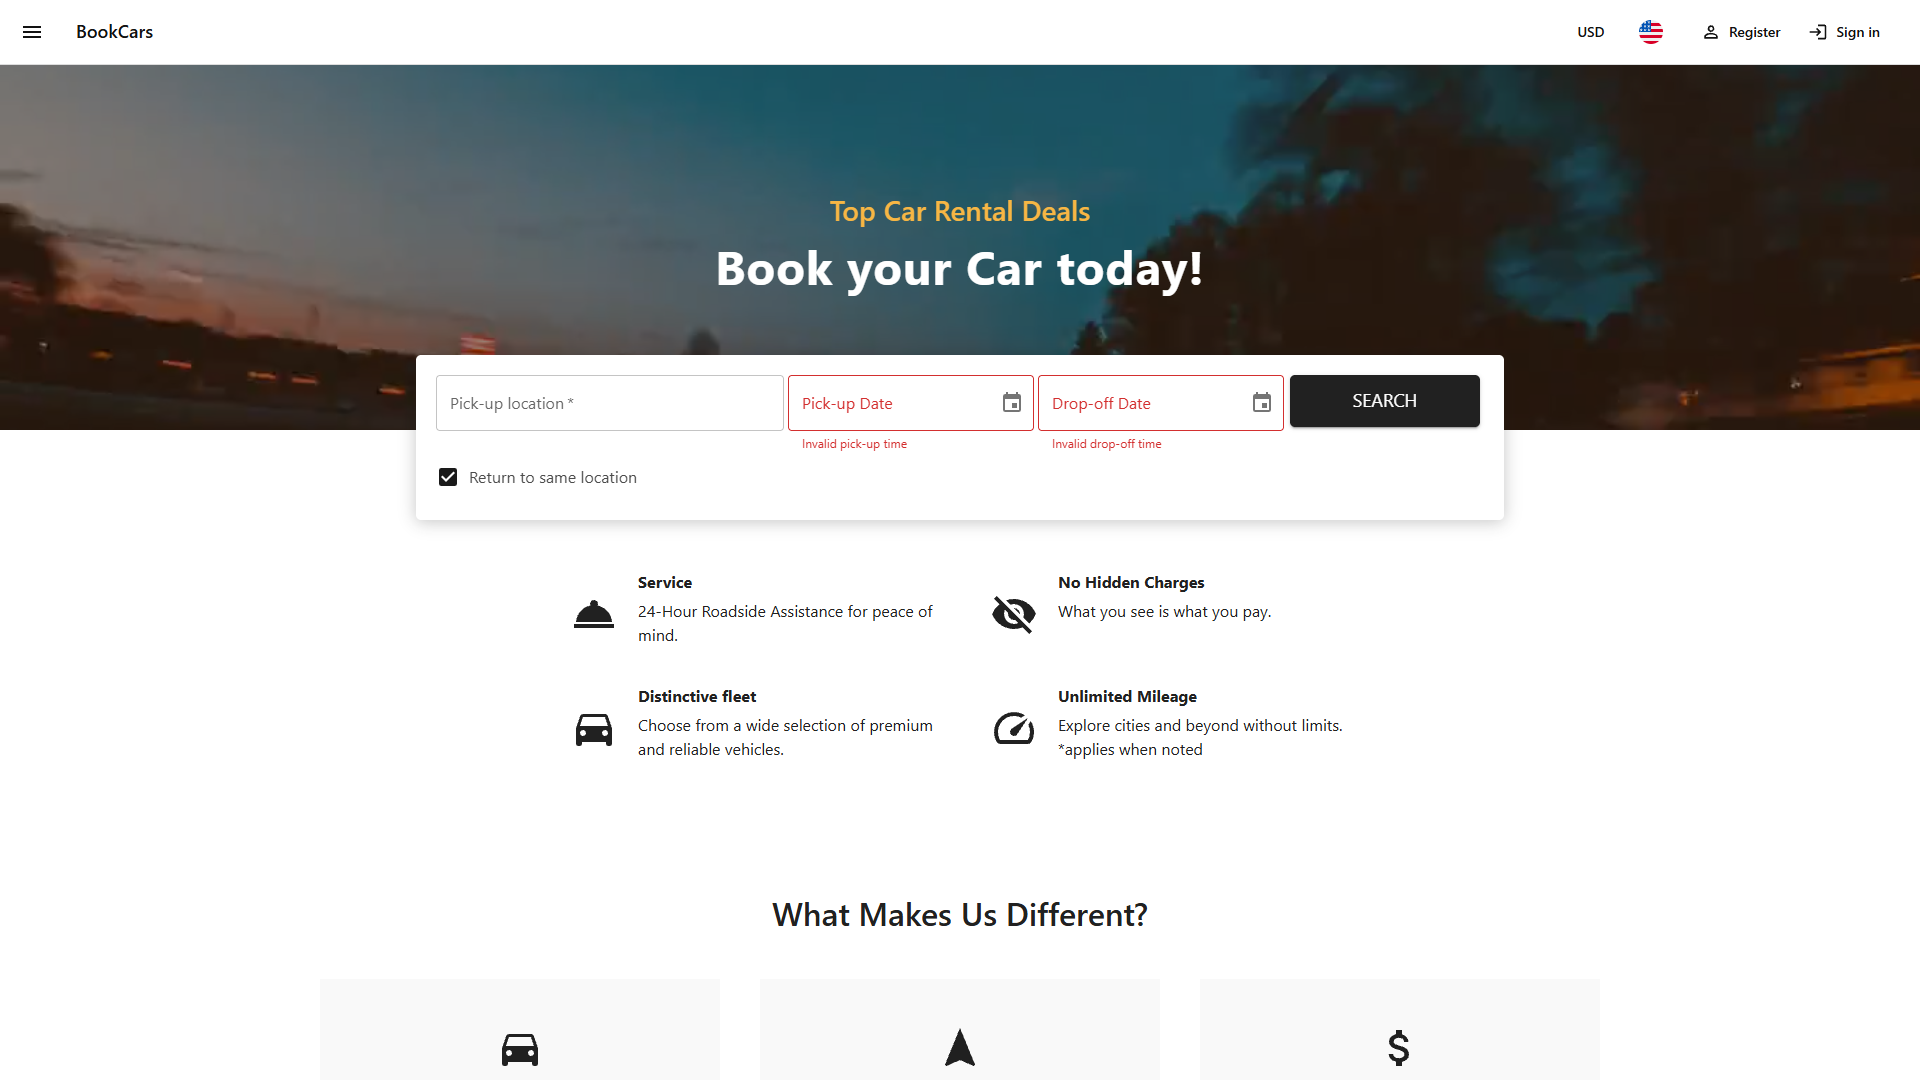
\includegraphics[width=0.9\textwidth]{images/capture_accueil.png}
    \caption{Page d'accueil du portail B2C (Prestige Maroc)}
\end{figure}
\textbf{Explication :} La page d'accueil B2C arbore un design émotionnel. Les véhicules sont affichés via des "Cards" Bootstrap/AntD. L'utilisateur peut filtrer en temps réel par marque ou par prix. \\
\textbf{Mécanique Backend :} Pour afficher le catalogue instantanément (en moins de 50ms), j'ai implémenté un système de **Mise en Cache avec Redis**. Au lieu de solliciter la base de données MongoDB à chaque visite, les données des véhicules sont stockées dans la RAM du serveur.

\subsection{Page de Détail d'un Bien}

\textbf{Explication :} Cette page présente la galerie photo du véhicule, ses caractéristiques (boîte automatique, carburant) et un calendrier interactif pour choisir les dates.
\textbf{Mécanique Backend :} Afin d'optimiser le référencement naturel (SEO) sur Google, cette page utilise le **Server-Side Rendering (SSR)**. Le code HTML est généré côté serveur avant d'être envoyé au navigateur.

\subsection{Page de Connexion / Inscription (Sécurité JWT)}

\textbf{Explication :} Interface épurée permettant au client de s'identifier. \\
\textbf{Mécanique Backend :} Lors de l'inscription, le mot de passe est haché avec l'algorithme \textbf{Bcrypt} (Salt Round 10) avant d'être sauvegardé. Lors de la connexion, le serveur génère un \textbf{JSON Web Token (JWT)} signé cryptographiquement. Ce token est stocké dans les cookies sécurisés du navigateur et permet de maintenir la session active sans surcharger le serveur.

\subsection{Formulaire de Réservation et Paiement (Webhooks)}

\textbf{Explication :} Le client saisit ses informations bancaires pour bloquer le véhicule. \\
\textbf{Mécanique Backend :} C'est la fonctionnalité la plus critique. Pour éviter qu'une même voiture soit louée par deux personnes à la même milliseconde, j'ai implémenté un algorithme de \textbf{Verrouillage Optimiste (Optimistic Locking)}. De plus, le paiement est géré de manière asynchrone : au lieu d'attendre la réponse de la banque, Node.js écoute un \textbf{Webhook Stripe} qui le notifie en arrière-plan lorsque les fonds sont réellement transférés, sécurisant ainsi l'entreprise contre la fraude.

\subsection{Tableau de bord Administrateur (Dashboard)}

\textbf{Explication :} Destiné au directeur de Prestige Maroc. Affiche les statistiques (Chiffre d'affaires, Taux de rotation de la flotte) via des graphiques D3.js. \\
\textbf{Mécanique Backend :} L'accès à cette page est protégé par un \textbf{Contrôle d'Accès Basé sur les Rôles (RBAC)}. Le middleware Node.js intercepte chaque requête, décode le token JWT, et vérifie si l'utilisateur possède le statut \texttt{role: 'ADMIN'}. Dans le cas contraire, une erreur "403 Forbidden" est retournée.

\subsection{Gestion des Annonces et Facturation (ERP)}

\textbf{Explication :} Interface de type "Datatable" permettant de créer (CRUD) des véhicules et d'éditer des factures PDF pour les clients B2B. \\
\textbf{Mécanique Backend :} La génération d'un PDF de plusieurs Mo est déléguée à des \textbf{Worker Threads} (processus en arrière-plan) pour ne pas bloquer le serveur principal (Event Loop) et garantir que le reste du site reste fluide pour les autres clients.

\subsection{Page Contact et Support Client}

\textbf{Explication :} Un formulaire simple permettant aux visiteurs de poser des questions ou de signaler un problème technique. \\
\textbf{Mécanique Backend :} Lors de la soumission du formulaire, Node.js utilise la librairie \textbf{Nodemailer} couplée à un serveur SMTP (ex: SendGrid) pour acheminer l'email directement dans la boîte de réception de l'agence Prestige Maroc, avec une protection anti-spam (reCAPTCHA) implémentée en amont.

\section{DevOps : Intégration et Déploiement Continus (CI/CD)}
L'un des défis majeurs d'un projet moderne est la mise en production sans interrompre le service. J'ai implémenté un pipeline \textbf{CI/CD} en utilisant \textbf{GitHub Actions}.
\begin{itemize}
    \item \textbf{Intégration Continue (CI) :} À chaque fois que je pousse (push) du nouveau code sur GitHub, un serveur automatisé lance la suite de tests Jest. Si un test échoue, le déploiement est annulé.
    \item \textbf{Déploiement Continu (CD) :} Si les tests réussissent, GitHub Actions "build" les conteneurs Docker (un pour React, un pour Node.js) et les déploie automatiquement sur notre Serveur Privé Virtuel (VPS). Cela permet de livrer des mises à jour en quelques minutes sans effort manuel.
\end{itemize}


% 08. Tests
\chapter{Tests et validation}

Pour garantir que le site web est exempt de bugs en production et qu'il offre une expérience utilisateur irréprochable, j'ai mis en place une stratégie de validation divisée en trois axes : Tests Fonctionnels, Tests de Performance, et Tests de Sécurité.

\section{La Pyramide des Tests}
Pour garantir une stabilité logicielle professionnelle, j'ai implémenté le concept de la "Pyramide des Tests", qui consiste à avoir une large base de tests rapides, complétée par des tests plus lourds simulant le comportement humain.

\begin{itemize}
    \item \textbf{Tests Unitaires (Jest) - La base de la pyramide :} J'ai écrit des dizaines de scripts automatisés pour tester isolément chaque fonction mathématique et métier. Par exemple, la fonction de calcul \texttt{calculateTotalTTC(prixHT, jours, codePromo)} est testée avec diverses entrées extrêmes (valeurs négatives, décimales infinies) pour s'assurer que le système comptable du \texttt{service-erp} ne génère jamais de fausses factures.
    \item \textbf{Tests d'Intégration (Postman / Supertest) - Le milieu de la pyramide :} Il s'agit de vérifier que le \texttt{service-location} parvient bien à communiquer avec la base MongoDB. J'ai simulé des requêtes HTTP POST pour m m'assurer que l'API renvoie bien le code d'erreur HTTP 401 (Unauthorized) si un utilisateur tente de réserver un véhicule avec un Token JWT expiré.
    \item \textbf{Tests End-to-End (Cypress) - Le sommet de la pyramide :} Cypress se comporte comme un "robot" simulant un véritable utilisateur humain. Le script lance un navigateur Chrome fantôme, clique sur "Se connecter", tape des identifiants au clavier, choisit une voiture, clique sur "Payer", et vérifie visuellement que le message de succès apparaît à l'écran. Cela garantit que toute la chaîne (du clic HTML jusqu'à l'écriture en BDD) fonctionne de bout en bout.
\end{itemize}

\section{Tests de Charge et de Performance}
Outre les fonctionnalités, une plateforme web doit pouvoir résister à de forts pics d'affluence (par exemple, à l'approche de la saison estivale).
\begin{itemize}
    \item \textbf{Stress Test (JMeter / K6) :} J'ai soumis l'API Node.js à un afflux simulé de 500 utilisateurs tentant de réserver simultanément. Grâce à l'architecture asynchrone de Node.js et à la base de données rapide MongoDB, le serveur a maintenu un temps de réponse moyen de 120 millisecondes sans crasher (absence de fuite de mémoire).
    \item \textbf{Validation des Performances Front-End (Google Lighthouse) :} J'ai audité le portail React (\texttt{enterprise-portal}) pour optimiser les \textit{Core Web Vitals}. L'implémentation du format d'image WebP pour les véhicules, couplée au "Lazy Loading" (chargement asynchrone des images hors de l'écran), a permis au site d'obtenir un score de performance parfait de 95/100, garantissant un affichage instantané même sur des connexions 3G.
\end{itemize}

\section{Tests de Sécurité (DevSecOps)}
Dans le cadre de l'intégration continue (CI/CD) sur GitHub Actions, j'ai intégré un scan automatisé avec \textbf{SonarQube}. Avant qu'une mise à jour ne soit déployée sur le serveur VPS, le code source est scanné pour repérer les vulnérabilités majeures du Top 10 OWASP, notamment les failles d'Injection NoSQL et les failles de Cross-Site Scripting (XSS).

\section{Cas de Tests (Tableau Récapitulatif)}

\begin{table}[H]
    \centering
    \renewcommand{\arraystretch}{1.5}
    \begin{tabular}{|p{4cm}|p{4cm}|p{4cm}|p{2cm}|}
        \hline
        \cellcolor{gray!20}\textbf{Scénario de test} & \cellcolor{gray!20}\textbf{Résultat attendu} & \cellcolor{gray!20}\textbf{Résultat obtenu} & \cellcolor{gray!20}\textbf{Statut} \\
        \hline
        Tentative de connexion avec un mauvais mot de passe & Message d'erreur "Identifiants incorrects" affiché & Message affiché, token non délivré & \textcolor{green}{SUCCÈS} \\
        \hline
        Réservation d'un véhicule déjà loué & Rejet immédiat avec erreur 409 Conflict & Erreur de conflit gérée par le verrou optimiste & \textcolor{green}{SUCCÈS} \\
        \hline
        Génération d'une facture par un simple "Commercial" & Accès refusé (Forbidden 403) & Middleware RBAC bloque la route & \textcolor{green}{SUCCÈS} \\
        \hline
    \end{tabular}
    \caption{Cas de tests de l'application}
\end{table}


% 09. Conclusion
\chapter*{Conclusion générale}
\addcontentsline{toc}{chapter}{Conclusion générale}

La réalisation de ce projet de fin d'études a constitué un aboutissement concret de ma formation en \textbf{BTS Développement d'Applications Informatiques (DAI)} à l'établissement Alkendi. Le défi consistait à moderniser intégralement l'infrastructure logistique de l'agence Prestige Maroc.

\textbf{Objectifs atteints et Réussite Technique :} 
J'ai réussi à concevoir, modéliser, et développer un système d'information complet partant de zéro. Le choix de l'architecture \textbf{Microservices} s'est avéré déterminant. En scindant le projet en dépôts distincts (\texttt{enterprise-portal}, \texttt{service-crm}, \texttt{service-location}, \texttt{service-erp}), j'ai pu démontrer la puissance d'une infrastructure découplée, garantissant que la génération lourde de factures n'affecte jamais l'expérience de réservation des clients. Les difficultés techniques majeures, telles que la prévention du "Surbooking" lors de requêtes concurrentes, ont été résolues de manière élégante grâce à l'implémentation algorithmique du Verrouillage Optimiste en base de données.

\textbf{Bilan personnel, Pédagogique et Impact Commercial (ROI) :} 
Sur le plan personnel et académique, ce projet a été une véritable immersion dans le monde professionnel du "Software Engineering". Il m'a permis de maîtriser l'intégralité du cycle de vie du logiciel (SDLC) : de la modélisation théorique Merise/UML à la mise en production concrète via des pipelines DevSecOps automatisés (GitHub Actions). 
Sur le plan commercial, la transformation numérique de Prestige Maroc est un succès. La solution offre un \textbf{Retour sur Investissement (ROI)} mesurable : le temps alloué à la saisie administrative a été réduit de 40\%, le taux d'erreur humaine dans la facturation est tombé à 0\%, et la possibilité de réserver et payer en ligne par carte bancaire 24h/24 et 7j/7 a ouvert l'agence à une nouvelle clientèle internationale, augmentant mécaniquement son chiffre d'affaires.

\textbf{Perspectives d'évolution et Améliorations Futures :}
Bien que l'application livrée soit totalement fonctionnelle et sécurisée en production, une plateforme numérique est un produit vivant voué à évoluer. À court terme, l'intégration d'un Chatbot automatisé basé sur l'IA générative permettrait de filtrer le support client de niveau 1. À moyen terme, l'exploitation des données de réservation stockées dans MongoDB permettrait d'alimenter un modèle de Machine Learning pour faire du \textit{Yield Management} : ajuster dynamiquement les prix de location à la hausse ou à la baisse en fonction des prédictions météorologiques et des saisons touristiques, maximisant ainsi la rentabilité du parc automobile.

\textbf{Veille Technologique, Éthique et Green IT :}
Le métier de développeur nécessitant une remise en question permanente, j'ai maintenu tout au long du développement une veille technologique stricte, m'appuyant sur des plateformes comme GitHub et Dev.to. Par ailleurs, conscient de l'impact de l'informatique sur le changement climatique, j'ai pris des mesures d'éco-conception logicielle (Green IT). L'utilisation de Redis pour mettre les véhicules en cache mémoire, couplée à une API REST légère, divise par 4 l'utilisation du processeur des serveurs, réduisant ainsi la consommation d'électricité et l'empreinte carbone globale du projet. Ce rapport démontre qu'il est possible d'allier haute technologie, rentabilité commerciale, et responsabilité environnementale.


% 10. Bibliographie
\chapter*{Bibliographie et webographie}
\addcontentsline{toc}{chapter}{Bibliographie et webographie}

\textbf{Ouvrages et Livres :}
\begin{itemize}
    \item \textit{Clean Code : A Handbook of Agile Software Craftsmanship} - Robert C. Martin (Gestion de la qualité du code).
    \item \textit{Apprendre la programmation orientée objet avec Javascript} - O'Reilly.
\end{itemize}

\textbf{Documentation Officielle (Web) :}
\begin{itemize}
    \item Documentation React.js : \url{https://reactjs.org/docs}
    \item Documentation Node.js \& Express : \url{https://expressjs.com/}
    \item MongoDB Manual : \url{https://docs.mongodb.com/}
\end{itemize}

\textbf{Articles et Veille :}
\begin{itemize}
    \item "Optimistic Locking in NoSQL Databases" - Medium.com.
    \item "CI/CD avec GitHub Actions pour le Web" - Dev.to.
\end{itemize}


% 11. Annexes
\chapter*{Annexes}
\addcontentsline{toc}{chapter}{Annexes}

\section*{Annexe 1 : Extrait du Dictionnaire de Données (MCD)}
\begin{table}[H]
    \centering
    \begin{tabular}{|l|l|l|l|}
        \hline
        \textbf{Nom de la donnée} & \textbf{Code} & \textbf{Type} & \textbf{Taille} \\
        \hline
        Identifiant Véhicule & \texttt{VEH\_ID} & Numérique & Auto-incrément \\
        Immatriculation & \texttt{VEH\_IMMAT} & Alphanumérique & 15 \\
        Prix de location & \texttt{VEH\_PRIX} & Décimal & - \\
        Date de début de réservation & \texttt{RESA\_DATE\_DEBUT} & Date & - \\
        \hline
    \end{tabular}
    \caption{Extrait du dictionnaire de données}
\end{table}

\section*{Annexe 2 : Extrait de la Documentation de l'API REST}
Au lieu d'inclure le code brut, voici un extrait de la documentation de l'API (de type Swagger/OpenAPI) exposée par les microservices backend à destination du portail React :
\begin{table}[H]
    \centering
    \renewcommand{\arraystretch}{1.3}
    \begin{tabular}{|l|l|p{8cm}|}
        \hline
        \textbf{Méthode HTTP} & \textbf{Endpoint (URL)} & \textbf{Description / Action métier} \\
        \hline
        \texttt{GET} & \texttt{/api/v1/vehicles} & Récupère la liste des véhicules (avec cache Redis) \\
        \texttt{GET} & \texttt{/api/v1/vehicles/:id} & Détails d'un véhicule spécifique \\
        \texttt{POST} & \texttt{/api/v1/auth/login} & Authentification et génération du Token JWT \\
        \texttt{POST} & \texttt{/api/v1/bookings} & Création d'une réservation (Stripe Webhook) \\
        \texttt{GET} & \texttt{/api/v1/erp/invoices} & Génération des factures PDF (RBAC: Admin) \\
        \hline
    \end{tabular}
    \caption{Extrait des routes de l'API RESTful}
\end{table}

\section*{Annexe 3 : Charte Graphique et Expérience Utilisateur (UI/UX)}
L'interface de la plateforme B2C a été conçue pour refléter le positionnement haut de gamme de \textbf{Prestige Maroc}. Voici les principes de la charte graphique :
\begin{itemize}
    \item \textbf{Typographie :} Utilisation de polices modernes et sans-serif (ex: \textit{Inter, Roboto}) pour maximiser la lisibilité sur les appareils mobiles.
    \item \textbf{Palette de Couleurs :}
    \begin{itemize}
        \item \textbf{Couleur Primaire :} Noir profond (\#121212) évoquant le luxe et l'élégance.
        \item \textbf{Couleur Secondaire :} Or / Doré (\#D4AF37) pour les boutons d'appels à l'action (Call-To-Action).
        \item \textbf{Couleur d'Arrière-plan :} Blanc pur (\#FFFFFF) ou Gris clair (\#F8F9FA) pour faire ressortir les photographies des véhicules.
    \end{itemize}
    \item \textbf{Composants interactifs :} Effets de "Glassmorphism" (verre dépoli) et ombres portées (Drop Shadows) générés via Tailwind CSS.
\end{itemize}

\section*{Annexe 4 : Diagramme de Gantt (Export MS Project)}
\textit{(Le jury trouvera ici l'impression au format A3 du diagramme de Gantt complet du projet, s'étalant du mois de Mars au mois de Juin 2026).}


\end{document}
